\chapter{Introduction}

\section{Informaciones generales}
En los Viernes las clases son online y sincronas.

La asignatura se divide en does partes:
\begin{enumerate}
   \item Parte 1
   \begin{enumerate}
      \item[T1] Introducción
      \item[T2] Planificación inteligente\\
      Algunos ejemplos son la planificación de procesos/planes de producción, o la planificación de rutas de reparto y logística;
en general, aplicaciones incluyen sistemas de ayuda a la toma de decisiones y recomendación.
      \item[T3] Optimización inteligente
      Optimización de la logistica empresarial (horarios, recursos, personal, turnos de trabajo,\dots)
      \item[T4] Agentes inteligentes
      Sistemas multiagentes que tienen que negociar, coordinarse y cooperar para un objetivo común. Pero algo videojuegos donde existe una competición o cooperación entre agentes y se requiere una búsqueda de alternativas.
   \end{enumerate}
   \item Parte 2
   \begin{enumerate}
      \item[T5] Modelado de lenguaje y autómatas finitos
      \item[T6] Aprendizaje profundo
      \item[T7] Aprendizaje profundo para clasificación de texto
      \item[T8] Aprendizaje profundo para clasificación de imágenes
   \end{enumerate}
\end{enumerate}

\begin{figure}[htbp]
   \centering
   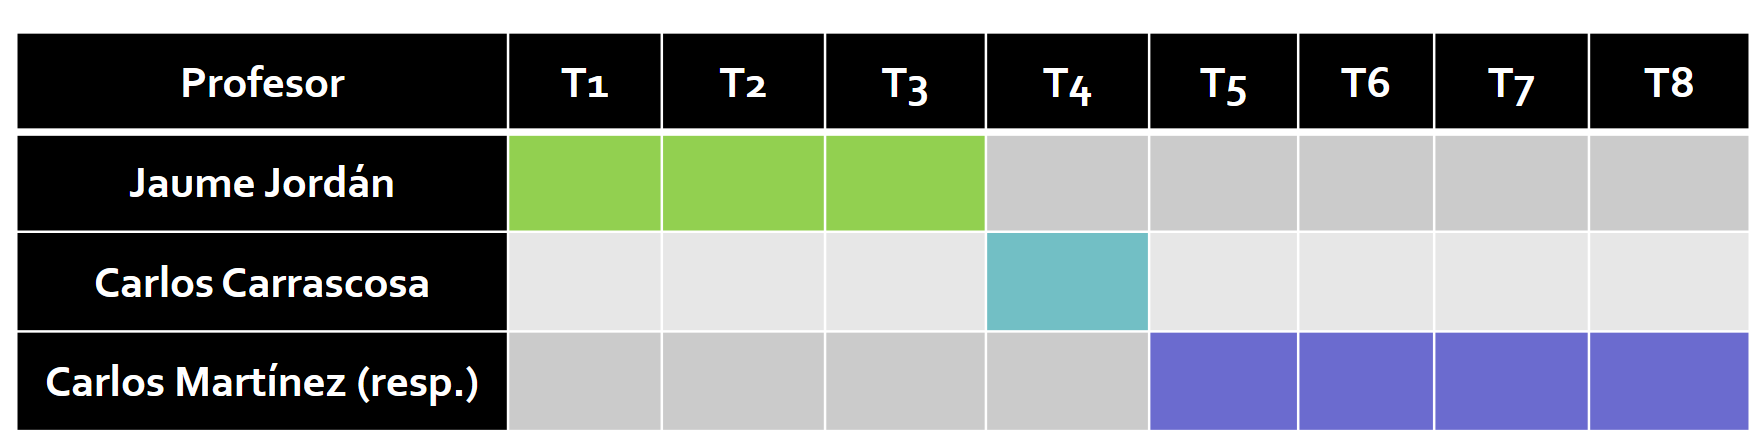
\includegraphics{images/01/profesores.png}
   \caption{Profesores}
   \label{fig:01/profesores}
\end{figure}

La evaluación se efectuará mediante:
\begin{itemize}
	\item Dos tests (\textbf{20 de junio a las 15:30}) sobre contenidos teóricos y
prácticos de la parte 1 (15\%) y parte 2 (15\%), totalizando 30\%.
	\item Trabajos académicos (70\%):
   \begin{itemize}
   	\item Parte 1 (35\%): tema 2 (15\%) y tema 4 (20\%).
	   \item Parte 2 (35\%): tema 5 (10\%), tema 7 (10\%) y tema 8 (15\%).
   \end{itemize}
\end{itemize}
\newpage

\section{Inteligencia Artificial}

\begin{paracol}{2}
   \colfill
   IA no es solo IA generativa. IA es un campo muy amplio que incluye otras cosas. Inicialmente se asociaba con el Machine Learning, pero ahora se ha ampliado a otras cosas.
   
   La Inteligencia Artificial es un campo interdisciplinario que implica máquinas capaces de imitar determinadas funcionalidades de la inteligencia humana, incluidas características como la percepción, el aprendizaje, el razonamiento, la resolución de problemas, la interacción\\lingüística e incluso la producción de trabajos creativos.
   \colfill

   \switchcolumn
   
   \begin{figure}[htbp]
      \centering
      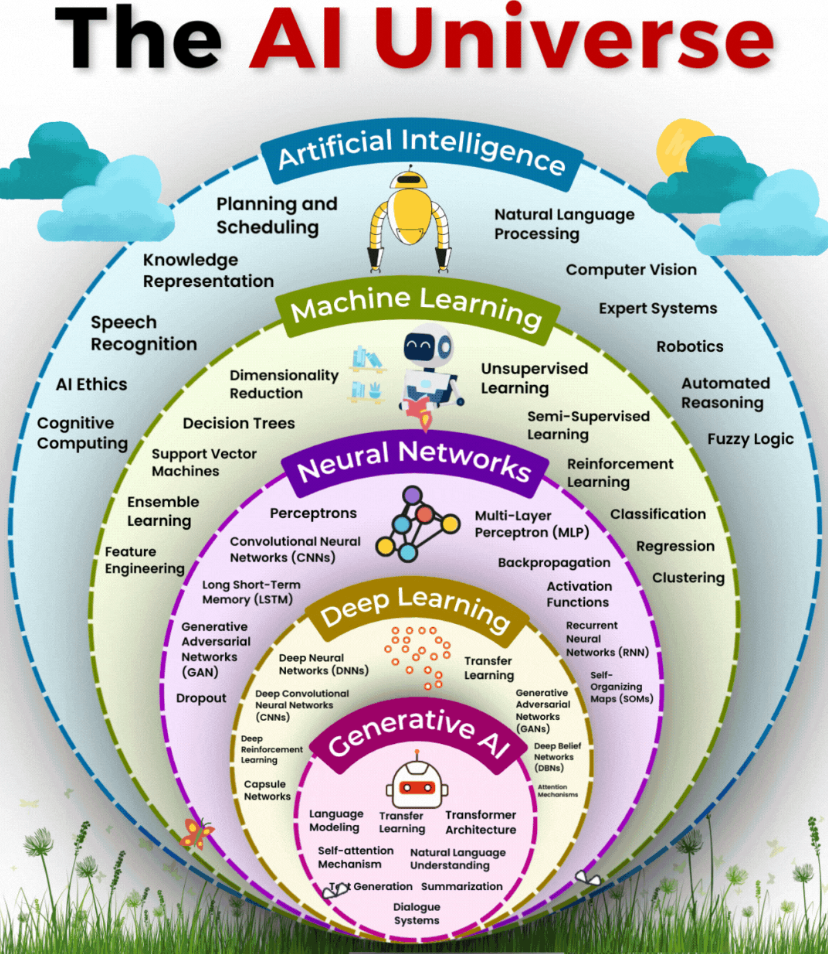
\includegraphics{images/01/AI.png}
      \caption{AI esquema. Según el profesor esto esquema no es completo, pero es cilustrativo.}
      \label{fig:01/AI}
   \end{figure}
\end{paracol}



{Modelos de IA:\ns
\begin{itemize}
	\item Aprendizaje supervisado
	\item Aprendizaje no supervisado
	\item Aprendizaje por refuerzo
\end{itemize}}

\subsection{Aplicaciones de la IA}
La Inteligencia artificial puede ser util para estas cosas:
Áreas y aplicaciones
\begin{itemize}
	\item Recuperación inteligente de la información
\begin{itemize}
	\item Recuperación de información no explícitamente representada
	\item Bases de datos deductivas. Procesos inferenciales. Sentido común. Interfaz natural
\end{itemize}
	\item Ingeniería del conocimiento (SBC y Sistemas Expertos)
\begin{itemize}
	\item Problemas NP: restricción de dominios, heurísticas y meta-heurísticas
	\item Planificación. Scheduling. Optimización. Sistemas de Ayuda a la Toma
de Decisiones

\end{itemize}
	\item Problemas (de búsqueda) combinatorios y de planificación
	\note{\ul{Este es el problema más importante de la IA}.}
\begin{itemize}
	\item Problemas NP: restricción de dominios, heurísticas y meta-heurísticas
	\item Planificación. Scheduling. Optimización. Sistemas de Ayuda a la Toma
de Decisiones
\end{itemize}
\item[] Hay también otras aplicaciones
\item Sistemas Multiagente y distribuidos que interactúan (cooperación)
\item Robótica
\item Percepción
\item Procesamiento de lenguaje natural
\end{itemize}


